\documentclass[12pt]{article}

\usepackage[margin=0.75in]{geometry}
\usepackage{graphicx}
\usepackage{float}

\newcommand{\graphwidth}{0.5\linewidth}

%\graphicspath{ {./res/image/}}


\title{ {\Huge Dual Rail Power Supply } \\
    ECE 302 Lab \#1 \\ LAD D11 / Bench \#9}
\author{
    Lyndon Sanche\\
    \texttt{lsanche@ualberta.ca}
    \and
    David Lenfesty\\
    \texttt{lenfesty@ualberta.ca}
}

\begin{document}
\pagenumbering{roman}

\maketitle


\section{Abstract}

Low-noise, low power split rail power supplies are a staple of the audio industry.
In order to generate the required audio waveforms for applications such as headphone or
low-power amplifiers, a negative and a positive voltage rail is necessary.

In this lab, a $\pm 10 V$ split rail power supply was implemented,
where the output ripple was designed to be less than $ 0.5 \% $ of the
regulated voltage. This supply operated using mains $115 V_RMS$, $60Hz $ power, with
a step down transformer leading to a diode rectifier. This rectifier supplied DC power to
positive and negative rails, each using a capacitor as a low-pass filter and implementing
a regulator output. The positive rail used an off the shelf 78L10AC linear regulator,
while the negative rail used a Zener diode-based regulator circuit.

\newpage
\pagenumbering{arabic}

\section{Objectives}

The objective of this lab is to design a split-rail power supply capable of supplying
$\pm 10V$ at 25mA, with a voltage error of less than 5\% and less than 0.5\% ripple.

This power supply will be used later in this lab to provide power for the audio amplifier
we will design.

\section{Design}

In order to simplify the design process, the power supply design was split into three
stages, rectification, filtering, and regulation. By splitting up the design into these
parts, it was simpler to test and easier to diagnose issues.

By simulating the circuit prior to building it, we were able to experiment wth different
component values and the effects of removing certain key components, which gave a better
understanding of how the circuit worked.

The purpose of this power supply is to take a 60Hz, 120Vrms signal, and convert it to a +-10V DC sige thagnal. The circuit is divided into
several stages for easier understanding. These stages include a transformer stage, rectifier stage, filter stage, and regulator stage. The combination 
of these stages allow us to convert a 120Vrms signal from a standard wall outlet, and convert it into two rails, one supplying roughly 10V and one supplying -10V. 
The supply is designed to have a minimal amount of ripple so the current going into the load does not flucuate.

The transformer stage is used to step down the 120Vrms voltage down to a voltage that will be manageable by the rectifier, filter, and regulator stages.

The rectiifer stage is the first part of converting our signal to positive and negative rails. We have chosen to use a bridge recitifier design as it converts all parts of the voltage signal 
to be positive or negative, depending on the rail. We have chosen the bridge rectifier instead of a rectifier design such as a half wave recitifer, as it doesn't cut out the negative parts of our wave, flipping them instead 
so we have more consistent voltage in our supply. We hook up the positive and negative rails to the same recitifer to produce a positive and negative recitified signal.

For the filter stage, we chose to use a shunt capacitor filter. The recitified AC signal that comes from the bridge rectifier is not appropriate to power electronic devices, so we use the capacitor filter to smooth out the output. We have chosen 
an appropriate size of capacitor to filter out a large amount of the AC components of our signal, leaving us a signal that stays around 10V with a manageable mount of ripple.

The regulator stage is different on the postive and negative rail. For the positive rail, we use a voltage regulator to remove the ripple on the signal, making it a near constant 10V dc signal. We find that the voltage regulator is very effective at removing 
ripple from our signal.

For the negative rail, we make use of a zener diode to regulate our voltage. Zener diodes are effective at regulating voltage when paired with the right ballast resistor. Even with the right ballast resistance, we were having some trouble removing the ripple from our signal, 
we put a capacitor in parallel with our load to regulate the voltage further. The result of this design is an effective voltage regulator, however, it is not as effective as a stand-alone voltage regulator.

After all these stages the power supply will output 10 volts on a postive and negative rail. These two rails will be useful when designing an audio amplifier, as audio needs both.

\section{Simulation}

\section{Results}


\section{Discussion}


The zener diode performs worse than the IC-based linear regulator. The linear regulator consumes less quiescent current to do the regulation,
and also has better ripple-rejection than the zener regulator.

While the zener diode required a small-sized ballast resistor and an extra capacitor on the output to reduce ripple,
the IC regulator did this without any extra compon

\section{Conclusion}

For this lab, a series of requirements was laid out for designing a power supply for an audio
amplifier. These requirements were taken and turned into a functional circuit that met
all of the requirements. In this lab, we were able to effectively use diodes to create
a functioning full-bridge rectifier, turning AC current into DC current, and then filter
and regulate this signal using a capacitors, an off-the-shelf voltage regulator IC, and
a zener diode.

\newpage

\begin{appendix}

\section{Rectifier Waveforms}

\subsection{Simulated}

\begin{figure}[H]
    \centering
    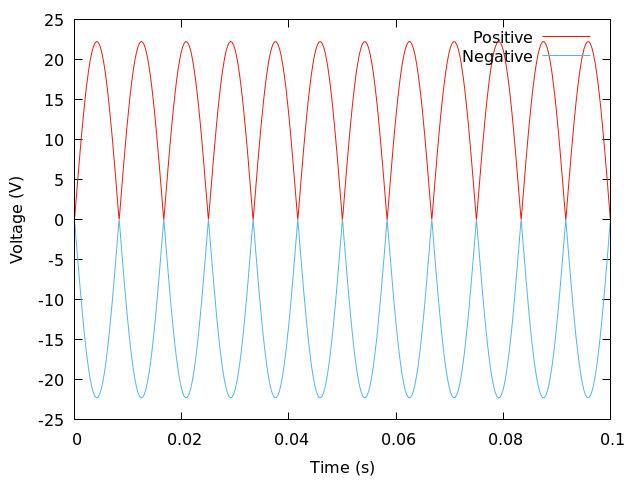
\includegraphics[width=\graphwidth]{./res/image/sim-rectifier-unfiltered.png}
    \caption{wbaiudbwiuabd}
    \label{sim:rectifier_unfiltered}
\end{figure}

\subsection{Measured}

\begin{figure}[H]
    \centering
    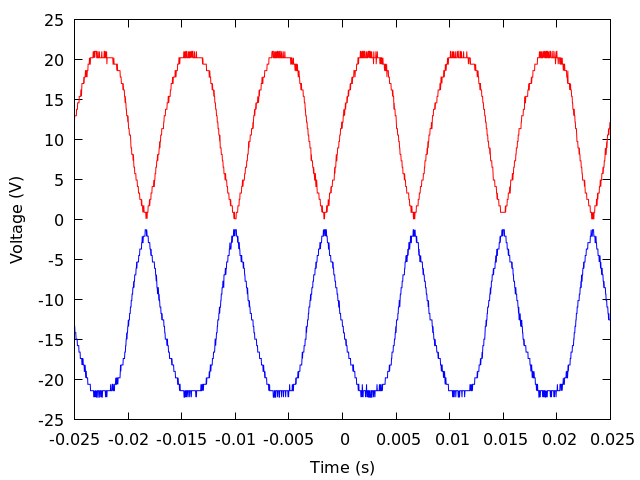
\includegraphics[width=\graphwidth]{./res/image/rectifier-output.png}
    \caption{wbaiudbwiuabd}
    \label{fig:rectifier_unfiltered}
\end{figure}

\section{Filter Waveforms}

\subsection{Simulated}

\begin{figure}[H]
    \centering
    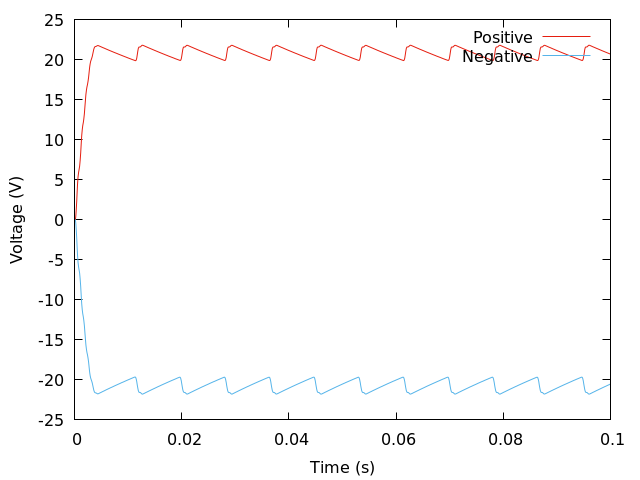
\includegraphics[width=\graphwidth]{./res/image/sim-filtered.png}
    \caption{abdiuwabdiu}
    \label{sim:filtered}
\end{figure}

\subsection{Measured}

\begin{figure}[H]
    \centering
    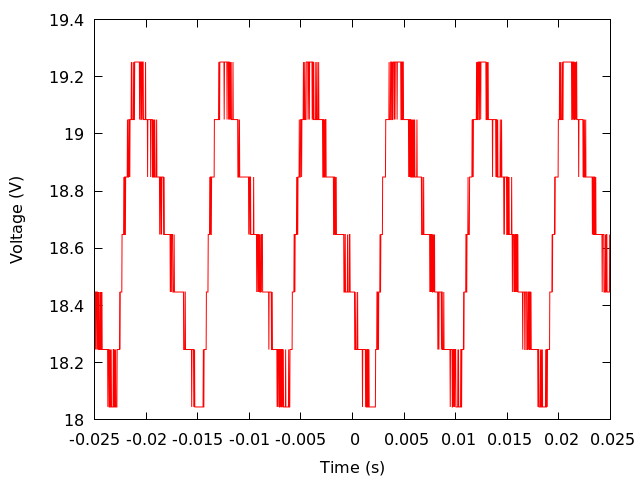
\includegraphics[width=\graphwidth]{./res/image/rectifier-withload.png}
    \caption{abdiuwabdiu}
    \label{fig:filtered}
\end{figure}

\section{Regulator Waveforms}

\subsection{Positive Regulator}

\subsubsection{Measured}

\begin{figure}[H]
    \centering
    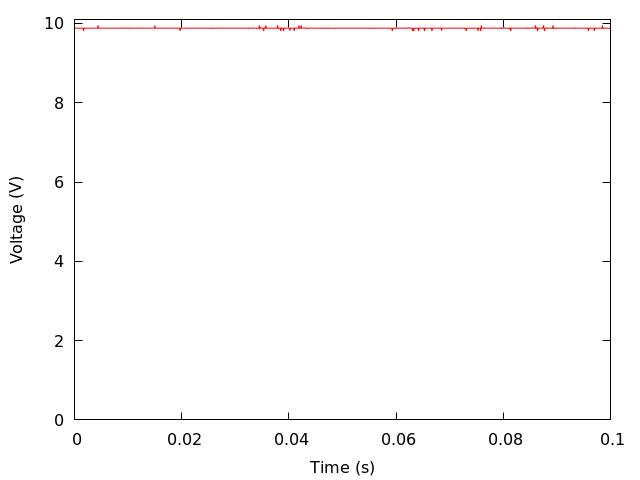
\includegraphics[width=\graphwidth]{./res/image/pos-fullload.png}
    \caption{abdiuwabdiu}
    \label{fig:pos_fullload}
\end{figure}

\begin{figure}[H]
    \centering
    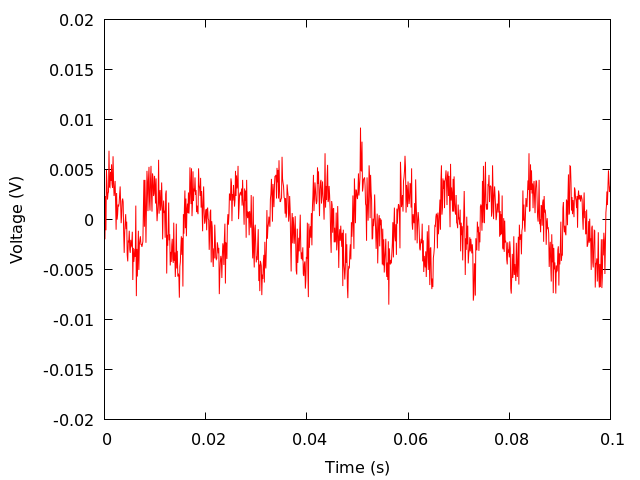
\includegraphics[width=\graphwidth]{./res/image/pos-fullload-ripple.png}
    \caption{abdiuwabdiu}
    \label{fig:pos_fullload_ripple}
\end{figure}

\begin{figure}[H]
    \centering
    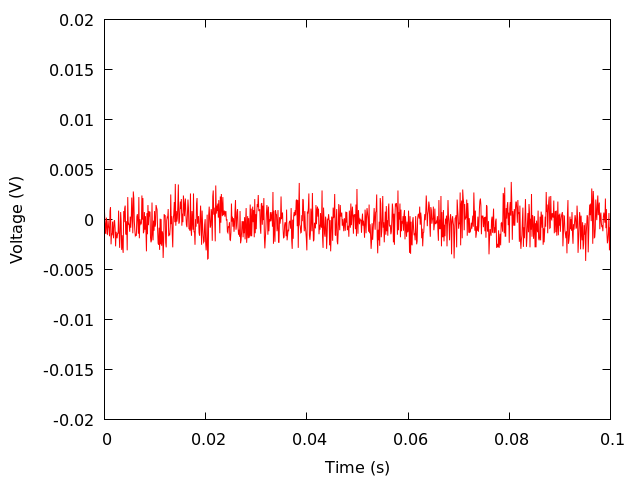
\includegraphics[width=\graphwidth]{./res/image/pos-noload-ripple.png}
    \caption{abdiuwabdiu}
    \label{fig:pos_noload_ripple}
\end{figure}

\subsection{Negative Regulator}

\subsubsection{Simulated}

\subsubsection{Measured}

\end{appendix}


\end{document}
